\chapter{Singular Homology}
\section*{Construction of the Singular Homology Functor}

Aim of this section is to construct for each $n \in \omega$ a functor $H_n : \mathsf{Top} \to \mathsf{AbGrp}$, called the \textit{$n$-th singular homology functor}.

\subsection*{Free Abelian Groups}

\begin{proposition}
	The forgetful functor $U : \mathsf{AbGrp} \to \mathsf{Set}$ admits a left adjoint.
	\label{prop:F_set_abgrp}
\end{proposition}

\begin{proof}
	We have to construct a functor $F : \mathsf{Set} \to \mathsf{AbGrp}$. Let $S$ be a set. Define 
	\begin{equation*}
		F(S) := \cbr[1]{f \in \mathbb{Z}^S : \supp f \text{ is finite}}.
	\end{equation*}
	Equipped with pointwise addition, $F(S)$ is an abelian group. There is a natural inclusion $\iota : S \hookrightarrow U\del[1]{F(S)}$ sending $x \in S$ to the function taking the value one at $x$ and zero else. Hence we may regard elements of $F(S)$ as formal linear combinations $\sum_{x \in S}m_x x$, where $m_x \in \mathbb{Z}$ for all $x \in S$. On morphisms $f : S \to T$ in $\mathsf{Set}$, define $F(f) : F(S) \to F(T)$ simply by setting $F(f)\del[1]{\sum_{x \in S}m_x x} := \sum_{x \in S}m_x f(x)$.\\	
	Let $G \in \ob(\mathsf{AbGrp})$ be an abelian group and $\varphi \in \mathsf{AbGrp}\del[1]{F(S), G}$ a morphism of groups. Define $\wbar{\varphi} \in \mathsf{Set}\del[1]{S,U(G)}$ by $\wbar{\varphi} := U(\varphi)$. Conversly, if we have $f \in \mathsf{Set}\del[1]{S,U(G)}$, define $\wbar{f} \in \mathsf{AbGrp}\del[1]{F(S),G}$ by $\wbar{f}\del[1]{\sum_{x \in S} m_x x} := \sum_{x \in S} m_x f(x)$. This is well defined since all but finitely many $m_x$ are zero and $G$ is abelian. It is easy to check that $\wbar{f}$ is indeed a morphism of groups. Let $\varphi \in \mathsf{AbGrp}\del[1]{F(S),G}$. Then
	\begin{align*}
		\wbar{\wbar{\varphi}}\del[4]{\sum_{x \in S} m_x x} &= \sum_{x \in S}m_x \wbar{\varphi}(x)\\
		&= \sum_{x \in S} m_x U(\varphi)(x)\\
		&= \sum_{x \in S} m_x \varphi(x)\\
		&= \varphi \del[4]{\sum_{x \in S} m_x x}.
	\end{align*}
	And for $f \in \mathsf{Set}\del[1]{S,U(G)}$ we have that
	\begin{equation*}
		\wbar{\wbar{f}}(x) = U(\wbar{f})(x) = \wbar{f}(x) = f(x). 
	\end{equation*}
	\noindent Hence $\wbar{\wbar{\varphi}} = \varphi$ and $\wbar{\wbar{f}} = f$ and so we have a bijection
	\begin{equation*}
		\mathsf{AbGrp}\del[1]{F(S),G} \cong \mathsf{Set}\del[1]{S,U(G)}.
	\end{equation*}
	The mapping $f \mapsto \wbar{f}$ will be referred to as \bld{extending by linearity}. To check naturality in $S$ and $G$ is left as an exercise.
\end{proof}

\begin{exercise}
	In proposition \ref{prop:F_set_abgrp}, check that $F : \mathsf{Set} \to \mathsf{AbGrp}$ is indeed a functor, called the \bld{free functor from $\mathsf{Set}$ to $\mathsf{AbGrp}$}, and the naturality of the bijection in both arguments. 
\end{exercise}

\begin{definition}[Free Abelian Group]
	Let $F : \mathsf{Set} \to \mathsf{AbGrp}$ be the free functor. For any set $S$, we call $F(S)$ the \bld{free group generated by $S$}.
\end{definition}

\subsection*{Chain Complexes}

\begin{definition}[Chain Complex]
	A \bld{chain complex} is a tuple $(C_\bullet,\partial_\bullet)$ consisting of a sequence $(C_n)_{n \in \mathbb{Z}}$ in $\ob(\mathsf{AbGrp})$ and a sequence $(\partial_n)_{n \in \mathbb{Z}}$ in $\mor(\mathsf{AbGrp})$, called \bld{boundary operators}, such that we have $\partial_{n} \in \mathsf{AbGrp}(C_n,C_{n - 1})$ and $\partial_n \circ \partial_{n + 1} = 0$ for all $n \in \mathbb{Z}$.
\end{definition}

\begin{definition}[Chain Maps]
	Let $(C_\bullet,\partial_\bullet)$ and $(C'_\bullet,\partial'_\bullet)$ be two chain complexes. A \bld{chain map $f_\bullet : C_\bullet \to C'_\bullet$} is a sequence $(f_n)_{n \in \mathbb{Z}}$ in $\mor(\mathsf{AbGrp})$ such that $f_n \in \mathsf{AbGrp}(C_n,C'_n)$ and the diagram
	\begin{center}
		\begin{displaymath}
			\xymatrix{ C_n \ar[r]^{\partial_n}\ar[d]_{f_n} & C_{n - 1} \ar[d]^{f_{n - 1}} \\
			C'_n \ar[r]_{\partial'_n} & C'_{n - 1}}
		\end{displaymath}
	\end{center}
	\noindent commutes for all $n \in \mathbb{Z}$.
\end{definition}

\begin{proposition}
	There is a category with objects chain complexes and morphisms chain maps.
	\label{prop:comp}
\end{proposition}

\begin{proof}
	Let $f_\bullet : C_\bullet \to C'_\bullet$ and $g_\bullet : C_\bullet' \to C_\bullet''$ be chain maps. Define a map $g_\bullet \circ f_\bullet$ by $g_n \circ f_n$ for each $n \in \mathbb{Z}$. This defines a chain map. Moreover, for each chain complex $C_\bullet$ define $\id_{C_\bullet}$ by $\id_{C_n}$ for all $n \in \mathbb{Z}$. It is easy to check, that then $\circ$ is associative and the identity laws hold.
\end{proof}

\begin{definition}[$\mathsf{Comp}$]
	The category in \ref{prop:comp} is called the \bld{category of chain complexes} and we refer to it as $\mathsf{Comp}$.
\end{definition}

\begin{theorem}
	There is a functor $\mathsf{Top} \to \mathsf{Comp}$.
	\label{thm:singular_complex}
\end{theorem}

\begin{proof}
	The proof is divided into several steps. Let us denote $C_\bullet : \mathsf{Top} \to \mathsf{Comp}$ for the claimed functor.
	\begin{enumerate}[label = \textit{Step \arabic*:},wide = 0pt, itemsep = 1.5ex]
		\item \textit{Construction of a sequence of abelian groups.} Let $v_0,\dots,v_k \in \mathbb{R}^n$ for some $n,k \in \omega$. We say that $(v_0,\dots,v_k)$ is \bld{affinely independent} if $(v_1 - v_0,\dots, v_k - v_0)$ is linearly independent. We define the \bld{k-simplex spanned by $(v_0,\dots,v_k)$}, written $\sbr[0]{v_0,\dots,v_k}$, to be
			\begin{equation}
				\textstyle{\sbr[0]{v_0,\dots,v_k} := \cbr[1]{\sum_{i = 0}^k s_i v_i : s_i \geq 0 \text{ for all } i = 0,\dots,k \text{ and } \sum_{i = 0}^k s_i = 1}}.
			\end{equation}
			\noindent equipped with the subspace topology. Moreover, we define the \bld{standard $n$-simplex $\Delta^n$} to be the $n$-simplex spanned by $(e_0,\dots,e_n)$ where $e_0 := 0 \in \mathbb{R}^n$ and $(e_1,\dots,e_n)$ is the standard ordered basis of $\mathbb{R}^n$. Let $X \in \ob(\mathsf{Top})$. Define a \bld{singular $n$-simplex in $X$} to be a morphism $\sigma \in \mathsf{Top}(\Delta^n,X)$. Let $n \in \mathbb{Z}$. Define
			\begin{equation}
				C_n(X) := \ccases{F\del[1]{\mathsf{Top}(\Delta^n,X)} & n \geq 0,\\
									0 & n < 0.}
			\end{equation}
			We will call elements of $C_n(X)$ \bld{singular $n$-chains}.
		\item \textit{Construction of boundary operators.} Let $X \in \ob(\mathsf{Top})$ and $\sigma$ a singular $n$-simplex in $X$ for $n \geq 1$. We define $\varphi^n_k : \Delta^{n-1} \to \Delta^n$, called the \bld{$k$-th face map}, to be the unique affine map determined by the vertex map
			\begin{equation*}
				\begin{matrix}
					& \varphi_k^n\\
					e_0 & \mapsto & e_0\\
					\vdots & & \vdots\\
					e_{k - 1} & \mapsto & e_{k - 1}\\
					e_k & \mapsto & e_{k + 1}\\
					\vdots & & \vdots\\
					e_{n - 1} & \mapsto & e_n.
				\end{matrix}
			\end{equation*}
			Explicitely, given $\sum_{i = 0}^{n - 1} s_i e_i \in \Delta^{n - 1}$, we have that (see \cite[152]{lee:topological_manifolds:2011})
			\begin{equation*}
				\varphi_k^n \del[4]{\sum_{i = 0}^{n - 1}s_i e_i} = \sum_{i = 0}^{n - 1}s_i \varphi_k^n(e_i).
			\end{equation*}
			Define now
			\begin{equation}
				\partial \sigma := \sum_{k = 0}^n (-1)^k \sigma \circ \varphi_k^n \in U\del[1]{C_{n - 1}(X)} 
			\end{equation}
			\noindent to be the \bld{boundary of $\sigma$}. Moreover, the \bld{singular boundary operator} is defined to be $\wbar{\partial_n}$ and $\partial_n := 0$ for $n \leq 0$.
		\item \textit{$\partial_n \circ \partial_{n + 1} = 0$ for all $n \in \mathbb{Z}$.} It is enough to consider $n \geq 1$, since $\partial_n \circ \partial_{n + 1} = 0$ holds trivially in the other cases. Let $X \in \ob(\mathsf{Top})$ and $\sigma \in \mathsf{Top}(\Delta^{n+1},X)$. Then we have
			\begin{align*}
				(\partial_n \circ \partial_{n + 1})(\sigma) &= \partial_n \del[4]{\sum_{k = 0}^{n + 1} (-1)^k \sigma \circ \varphi^{n + 1}_k}\\
				&= \sum_{k = 0}^{n + 1} (-1)^k \partial_n\del[1]{\sigma \circ \varphi^{n + 1}_k}\\
				&= \sum_{k = 0}^{n + 1}\sum_{j = 0}^n (-1)^{k + j} \sigma \circ \varphi^{n + 1}_k \circ \varphi^n_j\\
				&= \sum_{0 \leq k \leq j \leq n}(-1)^{k + j} \sigma \circ \varphi^{n + 1}_k \circ \varphi^n_j + \sum_{0 \leq j < k \leq n + 1}(-1)^{k + j} \sigma \circ \varphi^{n + 1}_k \circ \varphi^n_j\\
				&= \sum_{0 \leq j \leq k \leq n}(-1)^{k + j} \sigma \circ \varphi^{n + 1}_j \circ \varphi^n_k + \sum_{0 \leq j <k \leq n + 1}(-1)^{k + j} \sigma \circ \varphi^{n + 1}_k \circ \varphi^n_j\\
				&= \sum_{0 \leq j < k \leq n + 1}\del[1]{(-1)^{k + j - 1} \sigma \circ \varphi^{n + 1}_j \circ \varphi^n_{k - 1} + (-1)^{k + j} \sigma \circ \varphi^{n + 1}_k \circ \varphi^n_j}
			\end{align*}
			Since $\varphi_j^{n + 1} \circ \varphi_{k - 1}^n = \varphi_k^{n + 1} \circ \varphi_j^n$, it follows that
			\begin{equation*}
				\partial_n \circ \partial_{n + 1} = 0.
			\end{equation*}
			Indeed, consider the following chart of vertex maps:
			\begin{equation*}
				\begin{matrix}
					& \varphi_{k - 1}^n & & \varphi_j^{n + 1}\\
					e_0 & \mapsto & e_0 & \mapsto & e_0\\
					\vdots & & \vdots & & \vdots\\
					e_{j - 1} & \mapsto & e_{j - 1} & \mapsto & e_{j - 1}\\
					e_j & \mapsto & e_j & \mapsto & e_{j + 1}\\
					\vdots & & \vdots\\
					e_{k - 1} & \mapsto & e_{k - 1} & \mapsto & e_{k + 1}\\
					e_k & \mapsto & e_{k + 1} & \mapsto & e_{k + 2}\\
					\vdots & & \vdots\\
					e_{n - 1} & \mapsto & e_n & \mapsto & e_{n + 1}
				\end{matrix}
				\qquad\qquad\qquad
				\begin{matrix}
					& \varphi_j^n & & \varphi_k^{n + 1}\\
					e_0 & \mapsto & e_0 & \mapsto & e_0\\
					\vdots & & \vdots & & \vdots\\
					e_{j - 1} & \mapsto & e_{j - 1} & \mapsto & e_{j - 1}\\
					e_j & \mapsto & e_{j + 1} & \mapsto & e_{j + 1}\\
					\vdots & & \vdots\\
					e_{k - 1} & \mapsto & e_k & \mapsto & e_{k + 1}\\
					e_k & \mapsto & e_{k + 1} & \mapsto & e_{k + 2}\\
					\vdots & & \vdots\\
					e_{n - 1} & \mapsto & e_n & \mapsto & e_{n + 1}
				\end{matrix}.
			\end{equation*}
		\item \textit{Construction of chain maps.} Let $X,Y \in \ob(\mathsf{Top})$ and $f \in \mathsf{Top}(X,Y)$. For $n \geq 0$, define $f_n^\# : \mathsf{Top}(\Delta^n,X) \to U\del[1]{C_n(Y)}$ by $f^\# := f \circ \sigma$. Extending this map by linearity yields a homomorphism $f_n^\# : C_n(X) \to C_n(Y)$. Moreover, set $f_n^\# := 0$ for $n < 0$. Let $n \geq 1$ and $\sigma \in \mathsf{Top}(\Delta^n,X)$. Then on one hand we have
			\begin{equation*}
				(f_{n - 1}^\# \circ \partial_n)(\sigma) = f^\#_{n - 1}\del[4]{\sum_{k = 0}^n (-1)^k \sigma \circ \varphi^n_k} = \sum_{k = 0}^n (-1)^k f \circ \sigma \circ \varphi^n_k
			\end{equation*}
			\noindent and on the other
			\begin{equation*}
				(\partial_n \circ f^\#_n)(\sigma) = \partial_n(f \circ \sigma) = \sum_{k = 0}^n (-1)^k f \circ \sigma \circ \varphi^n_k.
			\end{equation*}
	\end{enumerate}
	Checking, that $C_\bullet$ is indeed a functor is left as an exercise.
\end{proof}

\begin{exercise}
	Show that $C_\bullet : \mathsf{Top} \to \mathsf{Comp}$ is a functor.
\end{exercise}

\subsection*{The Homology Functor}
\begin{proposition}
	For each $n \in \mathbb{Z}$ there exists a functor $\mathsf{Comp} \to \mathsf{AbGrp}$.
	\label{prop:homology_functor}
\end{proposition}

\begin{proof}
	Let $(C_\bullet,\partial_\bullet)$ be a chain complex. Let $x \in \im \partial_{n + 1}$. Hence there exists $y \in C_{n + 1}$ such that $x = \partial_{n + 1}y$. But then $\partial_nx = (\partial_n \circ \partial_{n + 1})(y) = 0$ and thus $\im \partial_{n + 1} \subseteq \ker \partial_n$. Define
	\begin{equation*}
		H_n(C_\bullet,\partial_\bullet) := \frac{\ker \partial_n}{\im \partial_{n + 1}} \in \ob(\mathsf{AbGrp}).
	\end{equation*}
	Let $(C_\bullet',\partial_\bullet')$ be a chain complex and $f_\bullet : C_\bullet \to C_\bullet'$ a chain map. Then $f_n(\ker\partial_n) \subseteq \ker \partial_n'$. Indeed, if $y \in f_n(\ker\partial_n)$, there exists $x \in \ker\partial_n$, such that $y = f_n(x)$. Since $f_\bullet$ is a chain map, we thus have $\partial_n'y = (\partial_n' \circ f_n)(x) = (f_{n - 1} \circ \partial_n)(x) = 0$. Moreover, we have that $\im \partial_{n + 1} \subseteq \ker \pi_n' \circ f_n$, where $\pi_n' : \ker \partial_n' \to H_n(C_\bullet',\partial_\bullet')$ is the usual projection. Indeed, if $y \in \im \partial_{n + 1}$, we find $x \in C_{n + 1}$, such that $y = \partial_{n + 1}x$. Since again $f_\bullet$ is a chain map, we have that $f_ny = (f_n \circ \partial_{n + 1})(x) = (\partial_{n + 1}' \circ f_{n + 1})(x) \in \im \partial_{n + 1}' = \ker \pi_n'$. Hence $\pi_n' \circ f_n$ factors uniquely through $\pi_n : \ker \partial_n \to H_n(C_\bullet,\partial_\bullet)$. Define $H_n(f_\bullet)$ to be this map. 
\end{proof}

\begin{remark}
	Let $(C_\bullet,\partial_\bullet)$ be a chain complex and $n \in \mathbb{Z}$. Then we will write $\langle x \rangle$ for an element in $H_n(C_\bullet,\partial_\bullet)$, the so-called \emph{homology class}. Hence if $(C_\bullet',\partial_\bullet')$ is another chain complex and $f_\bullet : C_\bullet \to C_\bullet'$ a chain map, then $H_n(f)\langle c \rangle = \langle f_nc\rangle$. 
\end{remark}

\begin{definition}[Cycles and Boundaries]
	Let $(C_\bullet,\partial_\bullet)$ be a chain complex and $n \in \mathbb{Z}$. Then elements of $\ker \partial_n$ are called \bld{$n$-cycles} and elements of $\im \partial_{n + 1}$ are called \bld{$n$-boundaries}.
\end{definition}

\begin{definition}[Homology Functor]
	Let $n \in \mathbb{Z}$ and $H_n : \mathsf{Comp} \to \mathsf{AbGrp}$ be the functor defined in proposition \ref{prop:homology_functor}. We call $H_n$ the \bld{n-th homology functor}.
\end{definition}

\begin{definition}[Singular Homology Functor]
	Let $n \in \mathbb{Z}$. The composition 
	\begin{equation}
		H_n \circ C_\bullet : \mathsf{Top} \to \mathsf{AbGrp}
	\end{equation}
	\noindent of the singular chain complex functor $C_\bullet$ in theorem \ref{thm:singular_complex} and the $n$-th homology functor of proposition \ref{prop:homology_functor} is called the \bld{singular homology functor}, written $H^{\mathrm{sing}}_n$.
\end{definition}

\begin{remark}
	For notational purposes we will often refer to the functor $H_n^{\mathrm{sing}}$ simply as $H_n$.
\end{remark}

\subsection*{First Properties of Singular Homolgy}

\begin{proposition}[Zeroth Singular Homology Group]
	Let $X \in \ob(\mathsf{Top})$ be non empty and path connected. Then $H_0(X) \cong \mathbb{Z}$.
\end{proposition}

\begin{proof}
	Since $\partial_0 : C_0(X) \to 0$, $\ker \partial_0 = C_0(X)$. Moreover, a map in $\mathsf{Top}(\Delta^0,X)$ can be identified with a point in $X$ and hence an element of $C_0(X)$ can be written as $\sum_{x \in X}m_x x$. Define a mapping $\Phi : C_0(X) \to \mathbb{Z}$ by $\Phi\del[1]{\sum_{x \in X}m_x x} := \sum_{x \in X}m_x$. This mapping is well defined since all but finitely many $m_x$ are zero. It is also easy to check, that $\Phi$ is a morphism of groups and that $\Phi$ is surjective. We claim that $\ker \Phi = \im \partial_1$. Indeed, if $\sum_{x \in X} m_x x \in \ker \Phi$, then $\sum_{x \in X}m_x = 0$. Let $p \in X$. Since $X$ is path connected, we find for each $x \in X$ a path $\sigma_x$ from $p$ to $x$. Consider the singular $1$-chain $\sum_{x \in X}m_x \sigma_x$. Then we have
	\begin{equation*}
		\partial_1 \del[4]{\sum_{x \in X}m_x \sigma_x} = \sum_{x \in X}m_x \del[1]{\sigma_x(1)- \sigma_x(0)} = \sum_{x \in X}m_x (x - p) = \sum_{x \in X} m_x x.
	\end{equation*}
	Hence $\sum_{x \in X}m_x x \in \im \partial_1$. Conversly, it is enough to show the claim on basis elements $\sigma \in \mathsf{Top}(\Delta^1,X)$. We have
	\begin{equation*}
		\Phi(\partial_1 \sigma) = \Phi\del[1]{\sigma(1) - \sigma(0)} = 1 - 1 = 0.
	\end{equation*}
	Hence the first isomorphism theorem \cite[23]{grillet:abstract_algebra:2007} implies that $H_0(X) \cong \mathbb{Z}$.
\end{proof}

\begin{proposition}[The Dimension Axiom]
	Let $\ast \in \ob(\mathsf{Top})$ be a one point space. Then $H_n(\ast) = 0$ for all $n \in \mathbb{Z}$, $n > 0$.
\end{proposition}

\section*{The Homotopy Axiom}

\begin{theorem}[The Homotopy Axiom]
	Let $f,g \in \mathsf{Top}(X,Y)$ be freely homotopic. Then $H_n(f) = H_n(g)$ for all $n \in \mathbb{Z}$.
\end{theorem}

\section*{The Hurewicz Theorem}
\subsection*{Abelianizations}

\begin{proposition}
	The forgetful functor $U : \mathsf{AbGrp} \to \mathsf{Grp}$ admits a left adjoint.
	\label{prop:Ab_grp_abgrp}
\end{proposition}

\begin{proof}
	Let $G \in \ob(\mathsf{Grp})$. For $g,h \in G$, define the \bld{commutator of $g$ and $h$}, written $\sbr[0]{g,h}$, by $\sbr[0]{g,h} := ghg^{-1}h^{-1}$. Moreover, set 
	\begin{equation*}
		X_G := \cbr[0]{\sbr[0]{g,h} : g,h \in G}
	\end{equation*}
	\noindent and define the \bld{commutator subgroup of $G$}, written $\sbr{G,G}$, by $\sbr{G,G} := \langle X_G \rangle$.

	\begin{lemma}
		For all $G \in \ob(\mathsf{Grp})$, $\sbr{G,G} \unlhd G$.
	\end{lemma}

	\begin{proof}
		We follow \cite[265]{lee:topological_manifolds:2011}. Clearly, $\sbr{G,G} \leq G$. By \cite[31]{karpfinger:algebra:2013} we have that 
	\begin{equation*}
		\langle X \rangle = \cbr[0]{x_1 \cdots x_n : n \in \omega \setminus \cbr{0}, x_1,\dots,x_n \in X_G \cup X^{-1}_G}.
	\end{equation*}
	It is easy to check that $X_G = X_G^{-1}$ and thus 
	\begin{equation*}
		\langle X \rangle = \cbr[0]{x_1 \cdots x_n : n \in \omega \setminus \cbr{0}, x_1,\dots,x_n \in X_G}.
	\end{equation*}
	Let $k \in G$ and $x_1 \cdots x_n \in \sbr{G,G}$. Since
	\begin{equation*}
		kx_1 \cdots x_n k^{-1} = kx_1 k^{-1} k x_2 k^{-1} k \cdots k x_n k^{-1}
	\end{equation*}
	\noindent it is enough to show that $k\sbr[0]{g,h}k^{-1} \in \sbr{G,G}$ for all $g,h \in G$. But this immediately follows from
	\begin{equation*}
		k\sbr[0]{g,h}k^{-1} = kghg^{-1}h^{-1}k^{-1} = \sbr[0]{kgk^{-1},khk^{-1}}.
	\end{equation*}
	Thus $\sbr{G,G} \unlhd G$.
	\end{proof}

	\begin{lemma}
		$G \in \ob(\mathsf{AbGrp})$ if and only if $\sbr{G,G} = \cbr{1}$.
		\label{lem:abelian_iff_commutator_trivial}
	\end{lemma}

	\begin{proof}
		Let $G \in \ob(\mathsf{AbGrp})$. Then $\sbr[0]{g,h} = 1$ for all $g,h \in G$, which implies $X_G = \cbr{1}$ and thus $\langle X_G \rangle = \cbr{1}$. Conversly, since $X_G \subseteq \sbr{G,G} = \cbr{1}$, we have that $\sbr[0]{g,h} = 1$ for all $g,h \in G$ which is equivalent to $gh = hg$ for all $g,h \in G$.	
	\end{proof}

	\begin{corollary}
		The quotient group $G/\sbr{G,G}$ is abelian.
	\end{corollary}

	\begin{proof}
		By lemma \ref{lem:abelian_iff_commutator_trivial} it is enough to show that $\sbr[0]{G/\sbr{G,G},G/\sbr{G,G}}$ is trivial. We actually show that $X_{G/\sbr[0]{G,G}} = \cbr{1}$. This immediately follows from
		\begin{equation*}
			\sbr[0]{g\sbr{G,G},h\sbr{G,G}} = ghg^{-1}h^{-1}\sbr{G,G} = \sbr{G,G}
		\end{equation*}
		\noindent for $g\sbr{G,G},h\sbr{G,G} \in G/\sbr{G,G}$.
	\end{proof}

	Hence define $\Ab : \mathsf{Grp} \to \mathsf{AbGrp}$ on objects by
	\begin{equation*}
		\Ab(G) := G/\sbr{G,G}.
	\end{equation*}
	The abelian group $\Ab(G)$ is called the \bld{abelianization of $G$}. On morphisms $\varphi : G \to H$ in $\mathsf{Grp}$ define $\Ab(\varphi) : \Ab(G) \to \Ab(H)$ by setting $\Ab(\varphi)(g\sbr{G,G}) := \varphi(g)\sbr{H,H}$. It is easy to check that this is a well defined morphism of abelian groups.\\
	Let $H \in \ob(\mathsf{AbGrp})$ and $\psi \in \mathsf{AbGrp}(\Ab(G),H)$. Define $\wbar{\psi} \in \mathsf{Grp}(G,U(H))$ by setting $\wbar{\psi}(g) := \psi(g\sbr{G,G})$. If $\varphi \in \mathsf{Grp}(G,U(H))$, define $\wbar{\varphi} \in \mathsf{AbGrp}(\Ab(G),H)$ by $\wbar{\varphi}(g\sbr{G,G}) := \varphi(g)$. It is easy to check that this mapping is actually well defined and that $\wbar{\wbar{\psi}} = \psi$ and $\wbar{\wbar{\varphi}} = \varphi$ holds.
\end{proof}

\begin{exercise}
	In proposition \ref{prop:Ab_grp_abgrp}, check that $\Ab : \mathsf{Grp} \to \mathsf{AbGrp}$ is indeed a functor and the naturality of the bijection in both arguments. 
\end{exercise}

\subsection*{The Hurewicz Morphism}
Since elements of $H_1(X)$ are homology classes of loops, one might suspect that there is a connection between the fundamental group $\pi_1(X,p)$ of a path connected space $X$ at $p$ and the first singular homology group $H_1(X)$. However, since $H_1(X)$ is always abelian and $\pi_1(X,p)$ is not necessarily abelian, they cannot be equal. In this section we use a little trick which makes matters simpler: if $c$ is any singular $n$-chain, not necessarily an $n$-cycle, we can also take its equivalence class modulo $n$-boundaries. We shall denote this class also with $\langle c \rangle$. Clearly, if $c$ is an $n$-cycle, then $\langle c \rangle$ is the usual homology class.

\begin{theorem}[Hurewicz Theorem]
	Let $X \in \ob(\mathsf{Top})$ be path connected and $p \in X$. Then $\Ab(\pi_1(X,p)) \cong H_1(X)$.
\end{theorem}

\begin{proof}
	We show the result in a sequence of lemmata.
	\begin{lemma}
		The mapping $h : \pi_1(X,p) \to H_1(X)$ defined by $h(\sbr{u}) := \langle u \rangle$ is well defined.
	\end{lemma}

	\begin{proof}
		First of all, since $u \in \Omega(X,p)$, we have that $u \in C_1(X)$. Moreover, $\partial u = u(1) - u(0) = p - p = 0$. Thus $u$ has a homology class $\langle u \rangle$. Let us check that $h$ is well defined. Suppose that $\sbr{u} = \sbr{v}$. Hence $F : u \simeq_{\partial I} v$. Consider the fundamental loop $\omega \in \Omega(\mathbb{S}^1,1)$. By \cite[70]{lee:topological_manifolds:2011}, $\omega$ is a quotient map. Since $u,v \in \Omega(X,p)$, there exist $\wtilde{u},\wtilde{v} \in \mathsf{Top}(\mathbb{S}^1,X)$, such that $\wtilde{u} \circ \omega = u$ and $\wtilde{v} \circ \omega = v$ (see \cite[72]{lee:topological_manifolds:2011}). Since $I$ is a locally compact Hausdorff space \cite[107]{lee:topological_manifolds:2011} implies that $\omega \times \id_I$ is a quotient map. Thus $F$ passes to the quotient and yields a map $\wtilde{F} \in \mathsf{Top}(\mathbb{S}^1 \times I,X)$. Now it is easy to check that $\wtilde{F} : \wtilde{u} \simeq_{\cbr{1}} \wtilde{v}$. Thus an application of the homotopy axiom yields
		\begin{equation*}
			\langle u \rangle = \langle \wtilde{u} \circ \omega \rangle = H_1(\wtilde{u})\langle \omega \rangle = H_1(\wtilde{v})\langle \omega \rangle = \langle \wtilde{v} \circ \omega \rangle = \langle v \rangle.
		\end{equation*}
	\end{proof}

	\begin{lemma}
		Let $u$ be a path in $X$ from $p$ to $q$. Then $\langle \wbar{u}\rangle = - \langle u\rangle$.
		\label{lem:reverse_path_homology}
	\end{lemma}

	\begin{proof}
		From figure \ref{fig:additive_inverse}, we deduce that an appropriate definition of a singular $2$-simplex $\sigma$ would be
		\begin{equation*}
			\sigma(x,y) := u(x).
		\end{equation*}
		Indeed
		\begin{equation*}
			\partial \sigma = \wbar{u} - c_p + u 
		\end{equation*}
		\noindent and since $c_p$ is the boundary of $\sigma_p \in \mathsf{Top}(\Delta^2,X)$ defined by $\sigma_p(x,y) := p$, we have that $\wbar{u} + u$ is a boundary.
		\begin{figure}[h!tb]
			\centering
			\begin{subfigure}[b]{.4\textwidth}
				\centering
				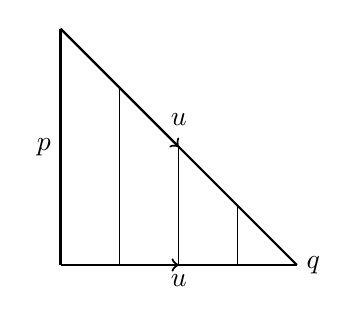
\begin{tikzpicture}[scale = 3]
					\draw [thick] (0,0) -- (1,0);
					\draw [thick] (0,0) -- (0,1);
					\draw [thick] (0,1) -- (1,0);
					\draw [thick,->] (0,0) -- (.5,0);
					\draw [thick,->] (0,1) -- (.5,.5);
				
					\draw [thin] (.25,0) -- (.25,.75);
					\draw [thin] (.5,0) -- (.5,.5);
					\draw [thin] (.75,0) -- (.75,.25);

					\draw (.5,0) node[below] {$u$};
					\draw (.5,.55) node[above] {$u$};
					\draw (0,.5) node[left] {$p$};
					\draw (1,0) node[right] {$q$};
				\end{tikzpicture}
				\caption{$\langle \wbar{u} \rangle = - \langle u \rangle$.}
				\label{fig:additive_inverse}
			\end{subfigure}
			~
			\begin{subfigure}[b]{.4\textwidth}
				\centering
				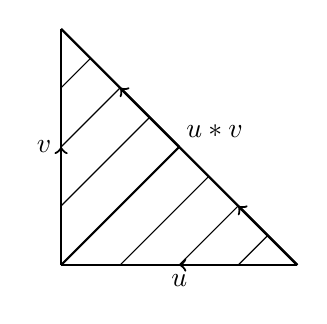
\begin{tikzpicture}[scale = 3]
					\draw [thick] (0,0) -- (1,0);
					\draw [thick] (0,0) -- (0,1);
					\draw [thick] (0,1) -- (1,0);
					\draw [thick] (0,0) -- (.5,.5);
					\draw [thick,->] (1,0) -- (.75,.25);
					\draw [thick,->] (.5,.5) -- (.25,.75);
					\draw [thick,->] (1,0) -- (.5,0);
					\draw [thick,->] (0,0) -- (0,.5);
				
					\draw [thin] (.25,0) -- (.625,.375);
					\draw [thin] (.5,0) -- (.75,.25);
					\draw [thin] (.75,0) -- (.875,.125);

					\draw [thin] (0,.25) -- (.375,.625);
					\draw [thin] (0,.5) -- (.25,.75);
					\draw [thin] (0,.75) -- (.125,.875);

					\draw (.5,0) node[below] {$u$};
					\draw (.65,.5) node[above] {$u \ast v$};
					\draw (0,.5) node[left] {$v$};
				\end{tikzpicture}
				\caption{$\langle u \ast v \rangle = \langle u \rangle + \langle v \rangle$.}
				\label{fig:hurewicz_homomorphism}
			\end{subfigure}
		\end{figure}
	\end{proof}

	\begin{lemma}
		Let $u$ and $v$ be paths in $X$ from $p$ to $q$ and from $q$ to $r$, respectively. Then $\langle u \ast v \rangle = \langle u \rangle + \langle v \rangle$.
		\label{lem:concatenation_addition}
	\end{lemma}

	\begin{proof}
		Consider figure \ref{fig:hurewicz_homomorphism}. The thin lines correspond to where $y - x$ is constant. Hence define $\sigma : \Delta^2 \to X$ by
		\begin{equation*}
			\sigma(x,y) := \ccases{
				u(y - x + 1) & 0 \leq y \leq x \leq 1,\\
				v(y - x) & 0 \leq x \leq y \leq 1.
			}
		\end{equation*}
		An application of the gluing lemma shows that $\sigma$ is actually a singular $2$-simplex. Moreover
		\begin{equation*}
			\partial \sigma = u \ast v - v + \wbar{u}.
		\end{equation*}
		Hence lemma \ref{lem:reverse_path_homology} yield
		\begin{equation*}
			0 = \langle u \ast v - v + \wbar{u}\rangle = \langle u \ast v \rangle - \langle v \rangle - \langle u \rangle.
		\end{equation*}
	\end{proof}

	\begin{corollary}
		$h$ is a morphism of groups.
		\label{cor:h_homomorphism}
	\end{corollary}

	\begin{corollary}
		Let $u,v,w$ be composable paths in $X$. Then $\langle (u \ast v) \ast w \rangle = \langle u \ast (v \ast w) \rangle$.
		\label{cor:composable_associative_homology}
	\end{corollary}

	\begin{lemma}
		$h$ is surjective.
	\end{lemma}

	\begin{proof}
		Let $x \in X$. If $x = p$, define $\gamma_p := c_p$. If $x \neq p$, by the path connectedness of $X$ we can choose a path $\gamma_x$ from $p$ to $x$. Hence we get a map $\gamma : X \to \mathsf{Top}(\Delta^1,X)$. Extending by linearity yields a mapping $\gamma : C_0(X) \to C_1(X)$. Let $c := \sum_{k = 1}^n m_k \sigma_k$ be a $1$-cycle in $X$. Consider
		\begin{equation*}
			\sbr{u} := \sbr[0]{\gamma_{\sigma_1(0)} \ast \sigma_1 \ast \overline{\gamma_{\sigma_1(1)}}}^{m_1} \cdots \sbr[0]{\gamma_{\sigma_n(0)} \ast \sigma_n \ast \overline{\gamma_{\sigma_n(1)}}}^{m_n} \in \pi_1(X,p). 
		\end{equation*}
		Now lemma \ref{lem:reverse_path_homology} and \ref{lem:concatenation_addition}, corollary \ref{cor:h_homomorphism} and \ref{cor:composable_associative_homology} yields
		\begin{align*}
			h(\sbr{u}) &= \sum_{k = 1}^n m_k \langle\gamma_{\sigma_k(0)} \ast \sigma_k \ast \overline{\gamma_{\sigma_k(1)}}\rangle\\
			&= \sum_{k = 1}^n m_k \del[1]{\langle\gamma_{\sigma_k(0)}\rangle + \langle\sigma_k\rangle + \langle \overline{\gamma_{\sigma_k(1)}}\rangle}\\
			&= \sum_{k = 1}^n m_k \del[1]{\langle\gamma_{\sigma_k(0)}\rangle + \langle\sigma_k\rangle - \langle \gamma_{\sigma_k(1)}}\rangle\\
			&= \langle c \rangle - \sum_{k = 1}^n m_k \langle \gamma_{\sigma_k(1) - \sigma_k(0)}\rangle\\
			&= \langle c \rangle - \sum_{k = 1}^n m_k \langle \gamma_{\partial \sigma_k}\rangle\\
			&= \langle c \rangle - \langle \gamma_{\partial c}\rangle\\
			&= \langle c \rangle.
		\end{align*}
	\end{proof}
	
\end{proof}


\section*{Applications}
\subsection*{The Brouwer Fixed Point Theorem}

\begin{definition}[Retract]
	Let $X \in \ob(\mathsf{Top})$ and $S \subseteq X$ a subspace. We say that \bld{$S$ is a retract of $X$},  if the inclusion $\iota : S \hookrightarrow X$ admits a retraction in $\mathsf{Top}$.
\end{definition}

\begin{lemma}
	Let $n \in \mathbb{Z}$, $n \geq 1$. Then $\mathbb{S}^n$ is not a retract of $\mathbb{B}^{n + 1}$. 	
\end{lemma}

\begin{proof}
	
\end{proof}

\begin{theorem}[Brouwer Fixed Point Theorem]
	Let $n \in \mathbb{Z}$, $n \geq 1$. Then every mapping $f \in \mathsf{Top}(\mathbb{B}^n,\mathbb{B}^n)$ has a fixed point.	
	\label{thm:brouwer_fixed_point}
\end{theorem}

\begin{proof}
	
\end{proof}
